\newpage
\section{Oral Arguments}

\vspace{5mm}
\begin{center}
    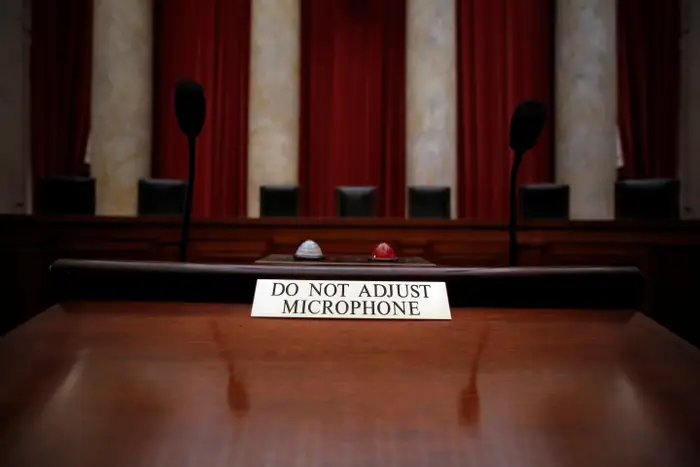
\includegraphics[width=350px]{images/oa_intro.png}\\[2mm]
    \footnotesize{Photo Credit: REUTERS/Jonathan Ernst}
\end{center}

\vspace{5mm}

\begin{center}
\begin{table}[H]
    \normalsize
    \centering
    \caption{What's Included (Oral Arguments)}
    \label{tab:oa_intro}
    \vspace{1mm}
    \begin{tabularx}{\textwidth}{>{\centering\arraybackslash}p{0.25\textwidth}>{\centering\arraybackslash}p{0.25\textwidth}>{\centering\arraybackslash}X}
        \toprule
        Area & Topic & Description \\
        \midrule
        Justice Participation & Justices (Words) & \RaggedRight Aggregate (term-level) bar chart and sitting-level breakdowns re: volume of words uttered by Justice. \\
        \addlinespace
        & Justices (Time) & \RaggedRight Aggregate bar chart and sitting-level breakdowns re: extent of time speaking by Justice. \\
        \addlinespace
        Attorney Participation & Attorneys (Words) & \RaggedRight Aggregate bar chart and sitting-level breakdowns re: volume of words uttered by arguing attorneys.  \\
        \addlinespace
        & Attorneys (Time) & \RaggedRight Aggregate bar chart and sitting-level breakdowns re: extent of time speaking by arguing attorneys. \\
        \addlinespace
        Justice-Attorney Interaction & Engagement & \RaggedRight Sitting-level breakdowns of Attorney-Justice interactions. \\
        \addlinespace
        Supplemental Information & Attorney Profiles & \RaggedRight Summary information on attorneys who argued during the 2024 Term. This includes statistics re: Supreme Court clerkships, demographics, experience in (or with) the Office of the Solicitor General (USG), and law school attendance \\
        \bottomrule
    \end{tabularx}
\end{table}
\end{center}
